%!TEX encoding = UTF-8 Unicode
\documentclass[a4paper]{article}

\usepackage{color}
\usepackage{url}
\usepackage[T2A]{fontenc} % enable Cyrillic fonts
\usepackage[utf8]{inputenc} % make weird characters work
\usepackage{graphicx}

\usepackage[english,serbian]{babel}


\usepackage[unicode]{hyperref}
\hypersetup{colorlinks,citecolor=green,filecolor=green,linkcolor=blue,urlcolor=blue}

\usepackage{listings}
\usepackage{float}



\begin{document}

\title{Informacioni sistem auto škole\\ \small{Seminarski rad u okviru kursa\\Informacioni sistemi\\ Matematički fakultet}}

\author{Emilija Stošić, emilijaz100sic@gmail.com \\ Mirko Ilić, ilicmirko07@gmail.com \\ Tamara Stojković, tamara.stojkovic.1998@gmail.com}

\date{4.~novembar 2022.}

\maketitle

\abstract{
  Osnovni cilj ovog projekta je demonstracija stečenog znanja na kursu ,,Informacioni sistemi’’ na master studijama na Matematičkom fakultetu u Beogradu. Mentori su profesor Saša Malkov i asistent Dara Milojković. Ideja je napraviti informacioni sistem auto škole, čija je namena da se vrši praćenje podataka i rezultata za kandidata od perioda upisa, do izdavanja vozačke dozvole. Pored kanidata postoji i evidencija o zaposlenim kadrovima u auto školi koji imaju određene uloge  u procesu evidencije i obuke kandidata. Rad obuhvata analizu sistema kroz slučajeve upotrebe: ,,Podnošenje zahteva za prijavu’’, ,,Teorijska obuka’’, ,,Praktična obuka’’, ,,Vođenje evidencije’’ i ,,Vođenje finansija’’. Postoji i prototip koji pokriva određene slučajeve upotrebe za ovaj rad.

}

\tableofcontents

\newpage

\section{Uvod}
\label{sec:uvod}

Osnovna namena ovog projekta je primena stečenog teorijskog i praktičnog znanja u izradi jednog informacionog sistema. Ideja je napraviti informacioni sistem auto škole, sa primarnim ciljem da se unapredi način na koji funkcionišu postojeći sistemi za neku auto školu. Pre svega uvodi se veći broj zaposlenih koji doprinose efikasnosti obuke kadnidata, rada zaposlenih i ostalih poslova u okviru škole. Uvode se razni online formulari, potvrde i ankete koje omogućavaju kandidatu da bude što zadovoljniji svojim procesom obuke, kao  i samoj auto školi za unapređenje poslovanja.
Svaka sekcija predstavlja jedan ili više zadataka koji su zadati od strane mentora.

\section{Analiza sistema}
\label{sec:naslov1}
 
Informacioni sistem je namenjen kandidatima tj. ljudima koji žele da završe vozačku obuku, kao i zaposlenima u toj auto školi. 
Sistem prikazuje način funkcionisanja jedne konkretne auto škole, a može se iskoristiti za unapređenje načina rada postojećih sistema u okviru auto škola.
U nastavku su opisani akteri koje smo prepoznali, kao i njihove uloge u ovom sistemu.

\
\subsection {Akteri}
\label{subsec:podnaslov1}
\begin{itemize}
\item \textbf{Administrator sistema} – Nalazi se na vrhu hijerarhije zaposlenih. Zadužen je direktno ili indirektno za većinu procesa u auto školi. Njegova uloga je takođe da održava bazu podataka. On vrši ažuriranje baze, dodavanjem novog klijenta kada dobije informacije od administrativnog radnika i šalje mejl potvrde kandidatu da je registrovan sa njegovim ID-jem i lozinkom.
\item \textbf{Administrativni radnik} – Na osnovu obrade podataka za prijavljenog kandidata formira kompletnu administrativnu dokumentaciju koja prati kandidata od upisa do izdavanja vozačke dozvole. Šalje podatke o kandidatu administratoru i kroz to zahteva njegovu registraciju u bazi podataka. Komunicira sa kandidatom i održava te podatke. Formira zapisnik teorijske i praktične provere.
\item \textbf{Računovođa} – Zadužen je za finansije. Vodi evidenciju o svim uplatama kandidata, o isplati plata zaposlenima i o održavanju cenovnika usluga.
\item \textbf{Nadležni za zapsolene} – Formira evidenciju kadrova(instruktora, predavača, računovođa, administrativnih radnika) i vodi računa o rasporedu rada. Vodi evidenciju o vozilima i opremi u auto školi.
\item \textbf{Predavači} – Održavaju časove, pripremaju materijale i kratke provere znanja. Imaju uvid o grupama i broju kandidata u svakoj grupi. Vode evidenciju o prisutnima na času predavanja.
\item \textbf{Instruktori} – Drže časove vožnje i vrše zakazivanje časova u dogovoru sa kandidatima. Upisuju u sistem podatke o održanom času. Imaju evidenciju o kandidatima koji su im dodeljeni. Vrše zapisnik o polaganju vozačkog ispita na kome su prisutni.
\item \textbf{Kandidati} – Prijavljuje se za obuku u auto školi  popunjavanjem online forme, unoseći svoje lične podatke i prilažući potrvdu o izvršenoj uplati. Na mejl dobija potvrdu da je registrovan i podatke za prijavu(ID i šifru). Na svom profilu može videti sve neophodne informacije, kao i proveriti ispravnost svojih podataka. Potrebno je da izvrši izbor grupe za teorijsku obuku. Nakon položene teorijske obuke, neophodno je da izabere instruktora i onda započinje praktičnu obuku. Časove zakazuje u dogovoru sa instruktorom, a neophodno je da se realizuje 40 časova praktične obuke(vožnje). Nakon toga, prijavljuje se za izlazak na vozački ispit odabirom željenog termina na formi. Ukoliko uspešno položi vozački ispit, neophodno je da popuni anketu o auto školi i dobija potvrdu o obavljenoj obuci u auto školi. U suprotnom, bira termin za novi izlazak na vozački ispit. 
\end{itemize}


\section{Slučajevi upotrebe}
\label{sec:podnaslov2}
U ovoj sekciji su predstavljeni slučajevi upotrebe (3 glavna, i slučajevi u okviru njih).
Za svaki slučaj upotrebe predstavljen je i odgovarajući dijagram aktivnosti, 
u okviru sekcije za taj pojedinačni slučaj upotrebe.
Za svaki glavni slučaj dodat je dijagram tog slučaja upotrebe, kao i odgovarajući BPMN dijagrami.
\subsection {Podnošenje zahteva za prijavu}
Proces registracije korisnika u auto školi započinje popunjavanjem online formulara, gde kandidat unosi svoje lične podatke. 
Administrativni radnik treba da proveri da kadnidat ispunjava potrebne uslove za upis i formira neophodnu dokumentaciju za kandidata. 
Nakon toga informacije prosleđuje administratoru sistema, koji unosi novog korisnika u bazu i prosleđuje dradniku ID i lozinku za trenutnog korisnika. 
Kada je kandidat prijavljen u auto školu, dobija imejl sa potvrdom o registraciji, svoj ID i lozinku , pa se može ulogovati na svoj nalog. 

\begin{figure}[H]
    \begin{center}
        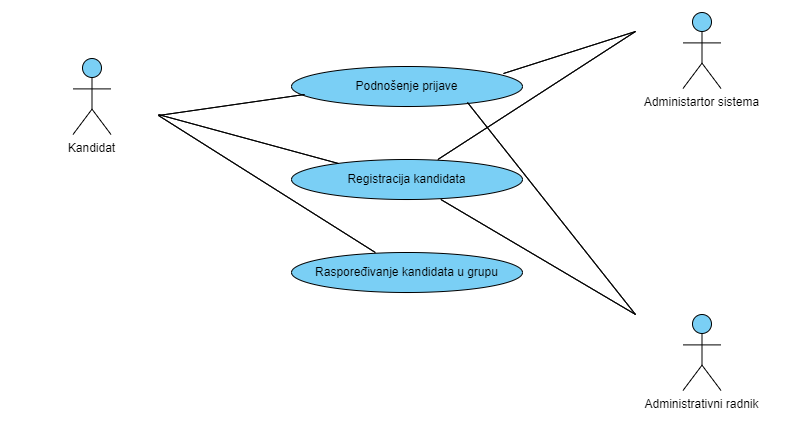
\includegraphics[width=140mm, height=65mm]{Diagrams/podnosenje_zahteva_za_prijavu.png}
    \end{center}
    \caption {Dijagram slučaja upotrebe - podnošenje zahteva za prijavu}
    \label{usecase_podnosenje_zahteva_za_prijavu}

\end{figure}

Na slici \ref{fig:stanja_kandidat_registracija} je prikazan dijagram stanja kandidata u procesu registracije.

\begin{figure}[H]
    \begin{center}
        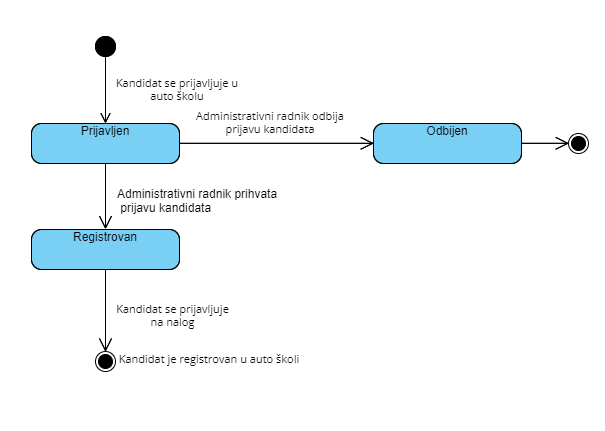
\includegraphics[width=130mm, height=60mm]{Diagrams/dijagram_stanja_registracija.png}
    \end{center}
    \caption {Dijagram stanja - podnošenje zahteva za prijavu}
    \label{fig:stanja_kandidat_registracija}

\end{figure}

\subsubsection{Podnošenje prijave}
\label{subsubsec:prijava}
\begin{itemize}
  \item \textbf{Kratak opis}: Da bi kandidat započeo obuku u auto školi, prvo mora da podnese prijavu za upis. Popunjava online formular, gde unosi svoje lične podatke, koji se nakon potvrde šalju administrativnom radniku. Radnik formira dokumentaciju za kandidata i prosleđuje ih administratoru sistema, koji unosi informacije o kandidatu u sistem.
  \item \textbf{Učesnici}: 
    \begin{itemize} 
      \item Kandidat
      \item Administrativni radnik
      \item Administrator sistema
    \end{itemize} 
  \item \textbf{Preduslovi}:
    \begin{itemize}
    \item Kandidat mora posedovati važeću ličnu kartu.
    \item Kandidat mora uplatiti prvu ratu.
    \end{itemize}
  \item \textbf{Postuslovi}:
      \begin{itemize}
      \item Kandidat ispunjava uslove za prijavu.
      \end{itemize}
  \item \textbf{Osnovni tok}:
      \begin{enumerate}
        \item Kandidat otvara online formu za prijavu u auto školu.
        \item Sistem prikazuje formu kandidatu.
        \item Kandidat popunjava formu, unoseći sve potrebne informacije.
        \item Kanidat šalje unete podatke klikom na dugme “Pošalji”.
        \item Sistem validira unos podataka.
        \item Sistem čuva podatke.
        \item Sistem prosleđuje podatke administrativnom radniku.
        \item Аdministrativni radnik proverava da li kanidat ispunjava uslove za upis.
        \item Administrativni radnik formira dokumentaciju za kandidata.
        \item Administrativni radnik prosleđuje podatke o kandidatu administratoru sistema.
      \end{enumerate}

  \item \textbf{Alternativni tokovi}:
      \begin{itemize}
        \item A1. \textbf{Kandidat ne ispunjava uslove za upis.}
        Ukoliko je u koraku 4 administrativni radnik uočio da kandidat ne ispunjava uslove za prijavu i kontaktira ga kako bi ga obavestio o tome i ispravio podatke ukoliko je moguće. Proces se nastavlja u 1. koraku osnovnog toka.
      \end{itemize}

  \item \textbf{Dodatne informacije}:\newline
  Potrebni podaci za prijavu su ime, prezime, JMBG, broj telefona, imejl adresa i potvrda o uplati prve rate.
\end{itemize}

\begin{figure}[H]
  \begin{center}
      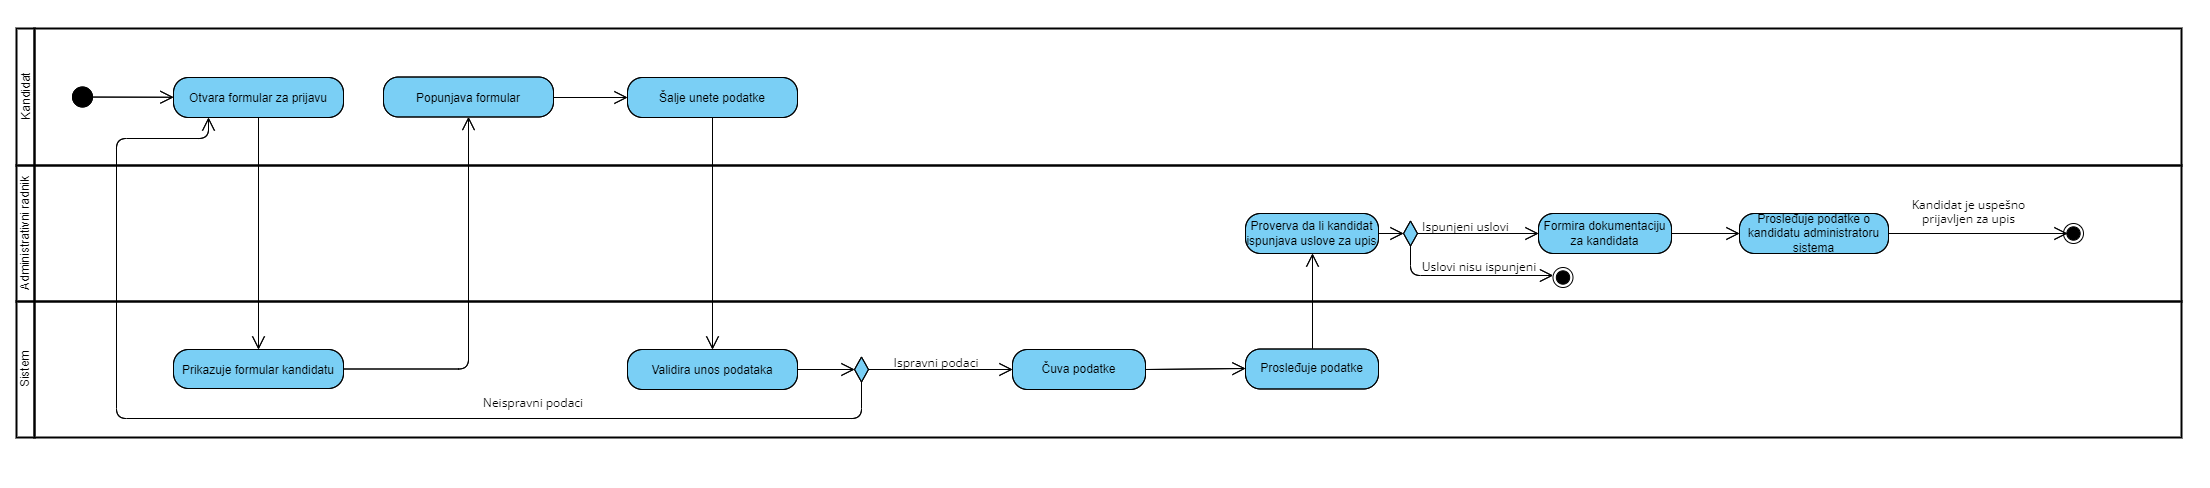
\includegraphics[width=140mm, height=70mm]{Diagrams/dijagram_aktivnosti_podnosenje_prijave.png}
  \end{center}
  \caption {Dijagram aktivnosti - Podnošenje prijave}
  \label{activity_podnosenje_prijave}

\end{figure}





\subsubsection{Registracija kandidata}
\label{subsubsec:registracija}
\begin{itemize}
  \item \textbf{Kratak opis}: Da bi kandidat mogao da se uloguje na svoj nalog i vidi svoje podatke, nepohodno je da dobije potvrdu da je upisan u auto školu, kao i nepohodan ID za logovanje.
  \item \textbf{Učesnici}:
  \begin{itemize}
    \item Kandidat
    \item Administrator sistema
    \item Administrativni radnik.
  \item \textbf{Preduslovi}:
    \begin{itemize}
    \item  Kandidat je popunio online prijavu.
    \item  Kandidat ispunjava uslove za upis.
    \end{itemize}
  \item \textbf{Postuslovi}:
      \begin{itemize}
      \item Kandidat je evidentiran u sistemu.
      \item Kandidat može da se prijavi na sistem.
      \end{itemize}
  \item \textbf{Osnovni tok}:
      \begin{enumerate}
        \item Administrator sistema prima informacije o novom kadnidatu.
        \item Administrator sistema unosi novog korisnika u bazu podataka.
        \item Sistem čuva unete podatke.
        \item Sistem šalje mejl novom kandidatu sa njegovim ID-jem.
        \item Sistem šalje mejl administrativnom radniku da je uspešno dodao novog kanidata.
        \item Administrativni radnik poziva kadnidata telefonom i proverava da li je dobio mejl sa svim potrebnim informacijama za prijavljivanje.
        \item Administrativni radnik ažurira spisak prijavljenih kandidata dodavanjem novog kadnidata.    
      \end{enumerate}

  \item \textbf{Alternativni tokovi}:
      \begin{itemize}
        \item A1. \textbf{Kandidat nije dobio mejl sa ID-jem i šifrom za pristupanje svom nalogu.}
        Ukoliko u koraku 4 kandidat nije dobio mejl, administrator sistema zahteva od sistema da ponovo pošalje mejl. Proces se nastavlja u koraku 4. osnovnog toka.
        \item A2. \textbf{Administrativni radnik ne može da kontaktira kadnidata.}
        Ukoliko u koraku 6 administrativni radnik ne može da stupi u kontakt sa kandidatom, trenutno stanje sistema se pamti i prekida se slučaj upotrebe na neko vreme. Naredni dan se slučaj upotrebe nastavlja ponovnim pozivom kandidata odnosno proces se nastavlja od 6. koraka osnovnog toka.
      \end{itemize}
\end{itemize}

\subsubsection{Raspoređivanje kandidata u grupu}
\label{subsubsec:grupe}
\begin{itemize}
  \item \textbf{Kratak opis}: Da bi kandidat bio raspoređen u grupu neophodno je da odabere neku od ponuđenih grupa, nakon logovanja na svoj nalog. 
  \item \textbf{Učesnici}: 
    \begin{itemize}
    \item  Kandidat - korisnik sistema koji bira grupu za teorijsku nastavu.
    \end{itemize}
  \item \textbf{Preduslovi}:
    \begin{itemize}
    \item Kandidat je dobio svoj ID i lozinku na mejl.
    \item Kandidat ima pristup internetu.
    \item Sistem je u funkciji.
    \end{itemize}
  \item \textbf{Postuslovi}:
      \begin{itemize}
      \item Kandidat je raspoređen u neku grupu.
      \end{itemize}
  
     
  \item \textbf{Osnovni tok}: 
      \begin{enumerate}
        \item Kandidat se prijavljuje na nalog.
        \item Kandidat klikom na dugme “Grupe” bira neku od ponuđenih grupa.
        \item Sistem šalje mejl kandidatu da je uspešno raspoređen u grupu i raspored održavanja časova.
        \item Kandidat dobija mejl sa podacima o grupi i rasporedu nastave.
      \end{enumerate}

  \item \textbf{Alternativni tokovi}:
      \begin{itemize}
        \item A1. \textbf{Neuspešno prijavljivanje.}
        Kandidat je pogrešio ID ili šifru u koraku 1, pa je nepohodno da proveri ispravnost podataka i da ih ponovo unese. Proces se nastvalja od koraka 1. osnovnog toka.
        \item A2. \textbf{Kandidat nije dobio mejl o raspoređivanju po grupama.}
        Kandidat nije raspoređen u željenu grupu, jer nije dobio mejl sa potvrdom u koraku 4, možda jer je vreme za prijavu isteklo (neko drugi je odabrao preostalo mesto). Proces se nastavlja od koraka 1. osnovnog toka.
      \end{itemize}


  \item \textbf{Specijalni zahtevi}:\newline
      Podaci koji su potrebni kako bi kandidat mogao da se uloguje su ID i lozinka u bazi.
\end{itemize}

  

\begin{figure}[H]
  \begin{center}
      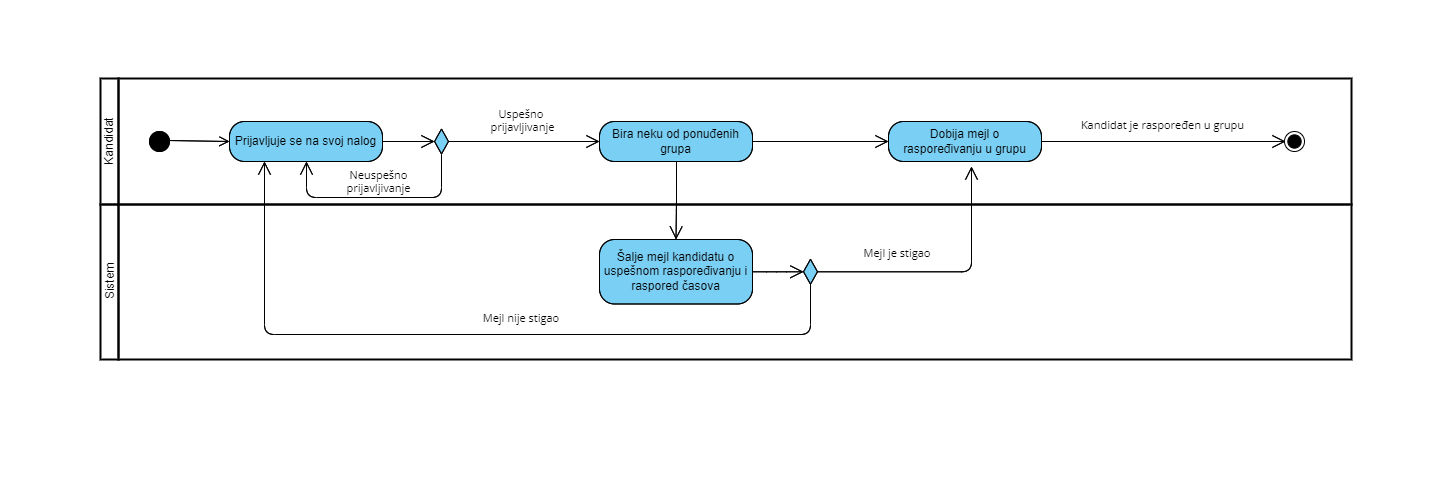
\includegraphics[width=140mm, height=70mm]{Diagrams/dijagram_aktivnosti_grupe.png}
  \end{center}
  \caption {Dijagram aktivnosti - Raspoređivanje kandidata u grupu}
  \label{activity_grupe}

\end{figure}


\begin{figure}[H]
    \begin{center}
        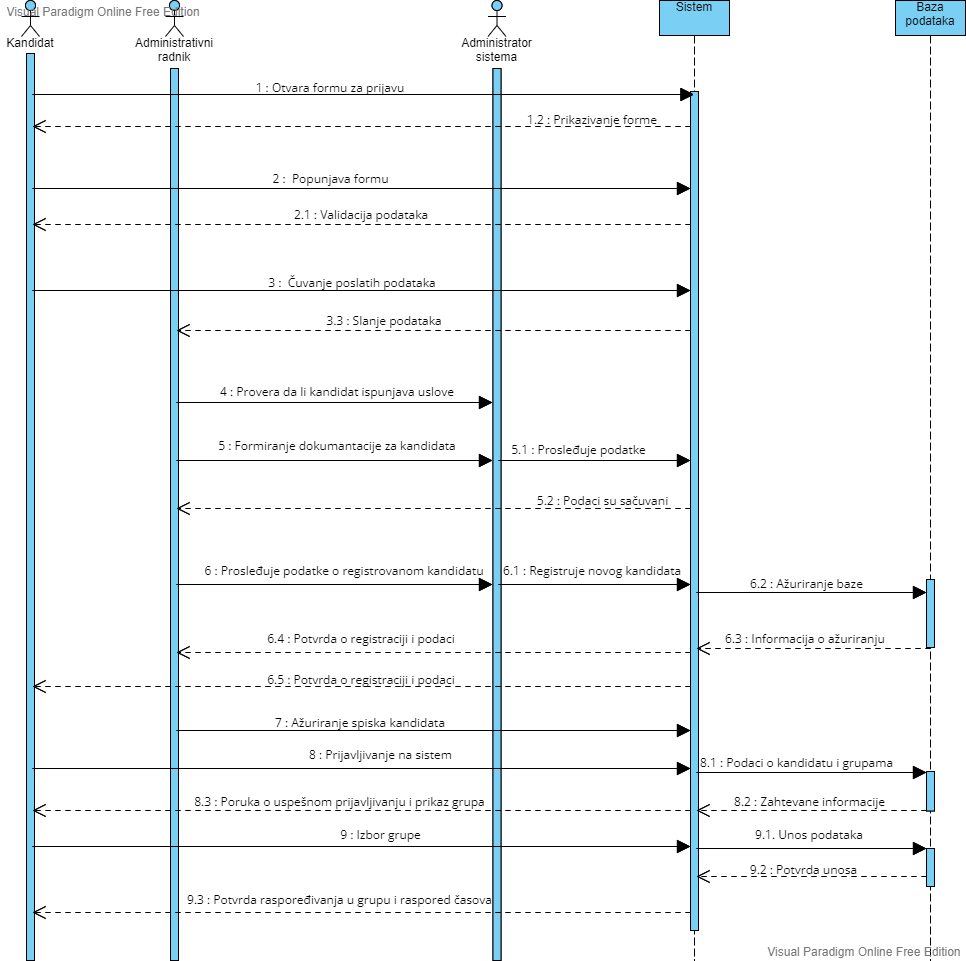
\includegraphics[width= 130mm]{Diagrams/dijagram_sekvence_podnosenje_zahteva.png}
    \end{center}
    \caption {Dijagram sekvenci - Podnošenje zahteva za prijavu}
    \label{fig:sekvenci_podnosenje_zahteva}

\end{figure}

Na slici \ref{fig:bpmn_podnosenje_zahteva} je prikazan BPMN dijagram procesa podnošenja zahteva za prijavu u auto školu,
koji predstavlja sled događaja u sistemu za 3 slučaja upotrebe:
\begin{itemize}
    \item Podnošenje prijave
    \item Registracija kandidata
    \item Raspoređivanje kandidata u grupu
\end{itemize}

\begin{figure}[H]
    \begin{center}
        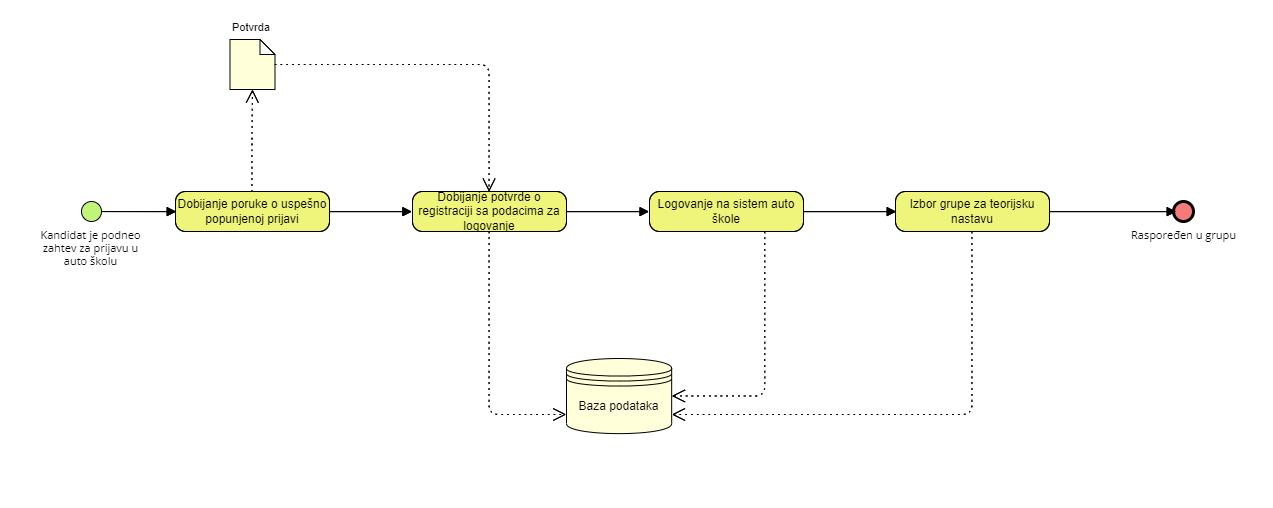
\includegraphics[width=155mm, height = 70mm]{Diagrams/bpmn_podnosenje_zahteva.png}
    \end{center}
    \caption {BPMN dijagram procesa podnošenja zahteva za prijavu}
    \label{fig:bpmn_podnosenje_zahteva}

\end{figure}


\subsection {Teorijska nastava}
Proces prijave za teorijsku nastavu kandidata, kao i vodjenje evidencije casova se odvija u okviru teorijske nastave. Takođe, tu imamo i evidenciju polaganja kandidata koji su uspesno prijavili svoj ispit i odslusali casove predavanja.

\begin{figure}[H]
  \begin{center}
      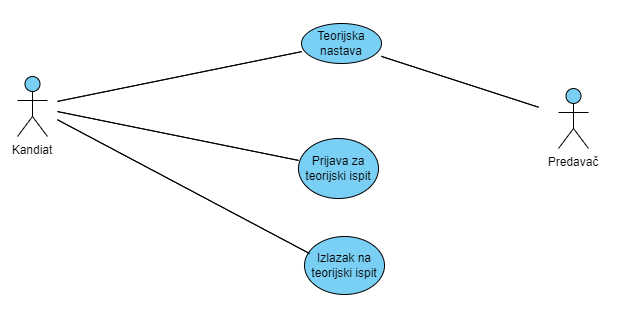
\includegraphics[width=140mm, height=70mm]{Diagrams/diagram teorijska nastava.png}
  \end{center}
  \caption {Teorijska nastava}
  \label{theory}

\end{figure}

\subsubsection{Teorijska nastava}
\label{subsubsec:prijava za nastavu}
\begin{itemize}
  \item \textbf{Kratak opis}: Kandidat koji se upisao u auto skolu pocinje sa pohadjanjem teorijske nastave u izabranoj grupi. Predavac evidentira prisustvo kandidata na casovima teorije koje on drzi.
  \item \textbf{Učesnici}:
    \begin{itemize}
    \item  Kandidat - korisnik sistema koji pohadja nastavu.
    \item  Predavac - korisnik koji drzi casove i evidentira prisustvo.
    \end{itemize}
  \item \textbf{Preduslovi}:
    \begin{itemize}
    \item  kandidat mora biti upisan u auto skolu.
    \item  kandidat mora biti rasporedjen u grupu kod predavaca.
    \item  kandidat je izmirio  prethodne troskove upisa.
    \item  predavac je zaduzen za grupu koju kandidati pohadjaju.
    \item  predavac je ulogovan na sistem.
    \item  sistem je dosutpan.
    \item  u sistemu ne postoji evidentiran cas za grupu u tekucem danu.
    \item  predavac  ima pristup internetu.
    \end{itemize}
  \item \textbf{Postuslovi}:
      \begin{itemize}
      \item Kandidat je evidentiran da je pohadjao nastavu.
      \item Predavac je evidnetirao odrzano predavanje.
      \end{itemize}
  \item \textbf{Osnovni tok}:
      \begin{enumerate}
        \item Predavac otvara stranicu za evidenciju prisustva korisnika.
        \item Predavac popunjava formular za zapocinjanje casa sa grupom.
        \item Predavac potvrdjuje da zapocinje cas sa grupom.
        \item Sistem prikazuje listu kandidata koji pohadjaju nastavu u toj grupi.
        \item Predavac evidentira prisustvo za svakog kandidata.
        \item Predavac zakljucuje evidenciju.
        \item Predavac zapocinje predavanje.
        \item Predavac nakon odrzanog cas zakljucuje cas.
        \item Sistem salje mail svim ucesnicima o uspeno zavrsenom casu i njihovom napretku.
      \end{enumerate}

  \item \textbf{Alternativni tokovi}:
      \begin{itemize}
        \item A1. \textbf{Neuspela validacija.}Ukoliku u koraku 2 sistem pronalazi neispravno polje formulara sistem obelezava polje koje treba ispraviti crvenom bojom, a ispod polja pise  uzrok neispravnosti. Nakon ponovnog ispravnog unosa podataka proces se nastavlja u koraku 3 osnovnog toka.s
      \end{itemize}
      
 \item \textbf{Dodatne informacije}:
      \begin{itemize}
        \item Polja formulara pri zapocinjanju cas su: Grupa, termin, cas.
      \end{itemize}
\end{itemize}

\subsubsection{Prijava za teorijski ispit}
\label{subsubsec:prijava za ispit}
\begin{itemize}
  \item \textbf{Kratak opis}: Kandidat nakon zavrsenog pohadjanja casova teorije podnosi prijavu za polaganje teorijskog ispita
  \item \textbf{Učesnici}:
    \begin{itemize}
    \item Kandidat korisnik sistema koji se prijavljuje za ispit
    \end{itemize}
  \item \textbf{Preduslovi}:
    \begin{itemize}
    \item  Kandidat mora biti upisan u auto skolu.
    \item  Kandidat je zavrsio-odslusao sve casove terojie.
    \item  Kandidat je izmirio prethodne troskove prijave.
    \item  Kandidat je ulogovan na sistem.
    \item  Sistem je dosutpan.
    \item  Kandidat ima pristup internetu.
    \end{itemize}
  \item \textbf{Postuslovi}:
      \begin{itemize}
      \item Kandidat je podneo prijavu za polaganje teorijskog ispita.
      \end{itemize}
  \item \textbf{Osnovni tok}:
      \begin{enumerate}
        \item Kandidat otvara stranicu za prijavu polaganja teorijskog ispita.
        \item Sistem prikazuje formular za prijavljivanje teorijskog ispita.
        \item Kandidata popunjava formular.
        \item Kandidat potvrdjuje prijavu klikom na dugme.
        \item Sistem evidnetira prijavu.
        \item Sistem salje mail kandidatu o uspesnoj prijavi.  
      \end{enumerate}

  \item \textbf{Alternativni tokovi}:
      \begin{itemize}
        \item A1. \textbf{Neuspela validacija.}
        Ukoliku u koraku 3 sistem pronalazi neispravno polje formulara sistem obelezava polje koje treba ispraviti crvenom bojom, a ispod polja pise  uzrok neispravnosti. Nakon ponovnog ispravnog unosa podataka proces se nastavlja u korakku 5.
      \end{itemize}
      
  \item \textbf{Dodatne informacije}:
      \begin{itemize}
        \item Polja formulara za prijavu: Ime, Prezime, JMBG, Datum poslednjeg casa, Predavac, Skenirana licna karata 
      \end{itemize}
\end{itemize}

\subsubsection{Izlazak na teorijski ispit}
\label{subsubsec:teorijski ispit}
\begin{itemize}
  \item \textbf{Kratak opis}: Kandidat koji je uspešno prijavio teorijski ispit izlazi na polaganje.
  \item \textbf{Učesnici}:
    \begin{itemize}
    \item Kandidat - korisnik sistema koji polaže ispit.
    \end{itemize}
  \item \textbf{Preduslovi}:
    \begin{itemize}
    \item  Kandidat mora biti upisan u auto školu.
    \item  Kandidat je odslušao sve časove teorije.
    \item  Kandidat je izmirio prethodne troškove prijave.
    \item  Kandidat je ulogovan na sistem.
    \item  Kandidat je uspešno prijavio teorijski ispit.
    \item  Sistem je u funkciji.
    \item  Kandidat ima pristup internetu.
    \end{itemize}
  \item \textbf{Postuslovi}:
      \begin{itemize}
      \item  Kandidat je je završio pohađanje teorijskog ispita.
      \end{itemize}
  \item \textbf{Osnovni tok}:
      \begin{enumerate}
        \item Kandidat je otvorio stranicu za polaganje teorijskog ispita.
        \item Sistem šalje na mail pristupnu lozinku za ispit.
        \item Kandidat unosi pristupnu lozinku.
        \item Sistem otvara stranicu sa teorijskim ispitom za kandidata.
        \item Kandidat potvrđuje da hoće da završi izradu ispita (ili je isteklo vreme za izvršavanje ispita).
        \item Sistem otvara stranicu sa rezultatima polaganja.
        \item Sistem šalje kandidatu mail sa ishodom polaganja za prijavu i rezultatima.
      \end{enumerate}

  \item \textbf{Alternativni tokovi}:
      \begin{itemize}
        \item A1. \textbf{Neuspela provera koda.}
        Neuspela provera koda: Ukoliko u koraku 3 kandidat unese loš pristupni kod polje za kod će postati crveno,
         i biće mu omogućeno da ponovo unese kod, ili da ponovno pošalje kod na mail. Kada ispravno unese kod proces se nastavlja u koraku 4.
      \end{itemize}
      
  \item \textbf{Specijalni zahtevi}:
      \begin{itemize}
        \item Polja formulara za prijavu: pristupni kod. 
      \end{itemize}
\end{itemize}

\begin{figure}[H]
  \begin{center}
      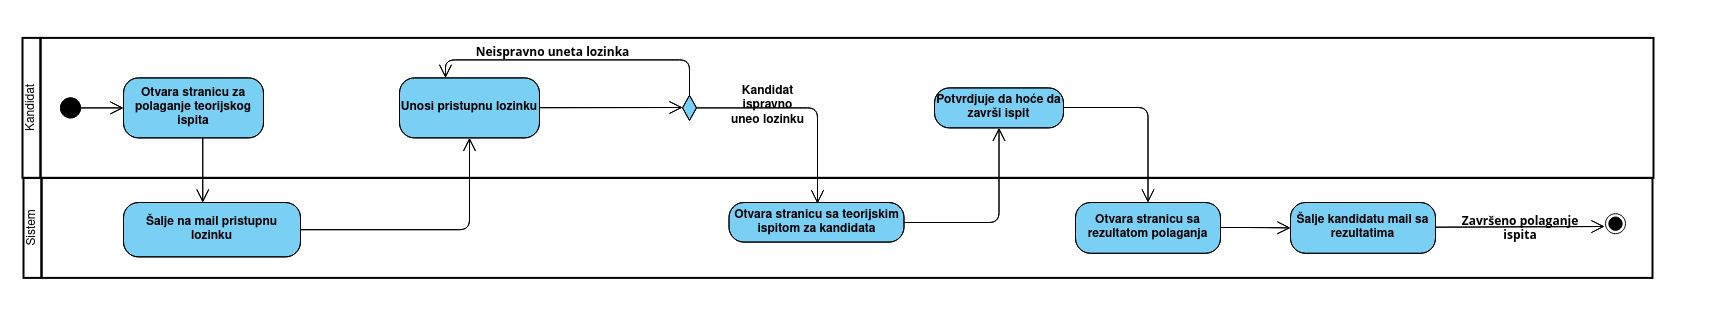
\includegraphics[width=140mm, height=70mm]{Diagrams/polaganje teorijskog ispita.png}
  \end{center}
  \caption {Dijagram aktivnosti - polaganje teorijskog ispita}
  \label{activity_polaganje_teorije}

\end{figure}


\subsection {Praktična nastava}
Proces praktične obuke započinje dostavljanjem auto školi potvrde o obavljenom lekarskom pregledu, koji kandidat mora da obavi. Neophodno je da kandidat odabere jednog od instruktora. Nakon 40 časova vožnje, i dobijene potvrde o položenoj prvoj pomoći, kandidat stiče uslov za prijavu za izlazak na vozački ispit. Kandidat se prijavljuje za ispit u jednom od ponuđenih termina i neophodno je da ima evidentirane potrebne uplate. Ukoliko je položio vozački ispit, pre izdavanja potvrde o položenom ispitu, neophodno je da kandidat popuni anketu o auto školi. Ovo će pomoći novim kandidatima, pre sve pri izboru odgovarajućeg instruktora.


\begin{figure}[H]
    \begin{center}
        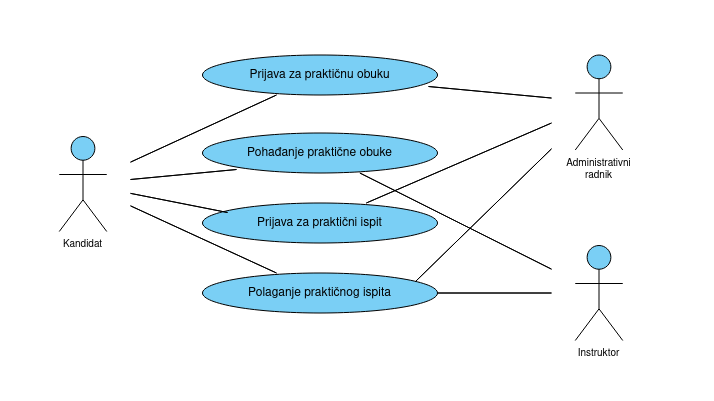
\includegraphics[width=107mm, height=60mm]{Diagrams/prakticna_obuka.png}
    \end{center}
    \caption {Praktična obuka}
    \label{usecase_praktična obuka}

\end{figure}

\subsubsection{Prijava za praktičnu obuku}

\vspace{3mm}

\begin{itemize}

\item \textbf{Kratak opis:} Da bi kandidat započeo praktičnu obuku potrebno je da se prijavi. Pre prijave kandidat dostavlja auto školi potvrde o obavljenom lekarskom pregledu, uplatama, nakon čega bira instruktora.

\vspace{2mm}

\item \textbf{Učesnici} \newline
   - Kandidat - korisnik sistema koji želi da se prijavi za praktičnu obuku.\newline 
   - Administrativni radnik - korisnik sistema koji proverava podatke, potvrđuje prijavu i šalje spisak instruktora.

\item \textbf{Preduslovi:} \newline
   - Sistem je u funkciji. \newline
   - Kadidat je položio teorijski ispit. \newline 
   - Kandidat je obavio lekarski pregled. 

\item \textbf{Postuslovi:} \newline
    - Kandidat se prijavio za praktičnu obuku 

\item \textbf{Osnovni tok:}  
   \begin{enumerate}
   \item Kandidat pristupa veb stranici i otvara formular za prijavu za praktičnu obuku.
   \item Sistem prikazuje formular.
   \item Kandidat popunjava formular.
   \item Kandidat klikom na dugme "Prijavi" šalje formular.
   \item Sistem evidentira prijavu.
   \item Sistem šalje podatke administrativnom radniku.
   \item Administrativni radnik proverava ispravnost i potpunost podataka.
   \item Administrativni radnik potvrdjuje prijavu i kandidatu šalje spisak slobodnih instruktora.
   \item Kandidat proverava mejl.
   \item Kandidat bira instruktora.
   \item Sistem belezi prijavu kandidata i izabranog instruktora.
   \end{enumerate}

\item \textbf{Alternativni tok:}  
   \begin{itemize}
   \item A1. \textbf{Neispravnost ili nepotpunost dokumentacije:}
  Ukoliko je u koraku 7 kandidat poslao nepotpun formular ili formular sadrži neke neispravne podatke, slučaj upotrebe se privremeno zaustavlja dok kandidat ne kompletira potrebnu dokumentaciju ili ispravi prosleđene podatke i proces se nastavlja od koraka 1 u osnovnom toku.
  \item A2. \textbf{Kandidat nije dobio mejl:}
  Ukoliko u koraku 9 kandidat nije dobio mejl o potvrdi prijave i spisak slobodnih instruktora, obaveštava administrativnog radnika i proces se nastavlja od koraka 8 u osnovnom toku.
   \end{itemize}

\end{itemize}  

\begin{figure}[H]
  \begin{center}
      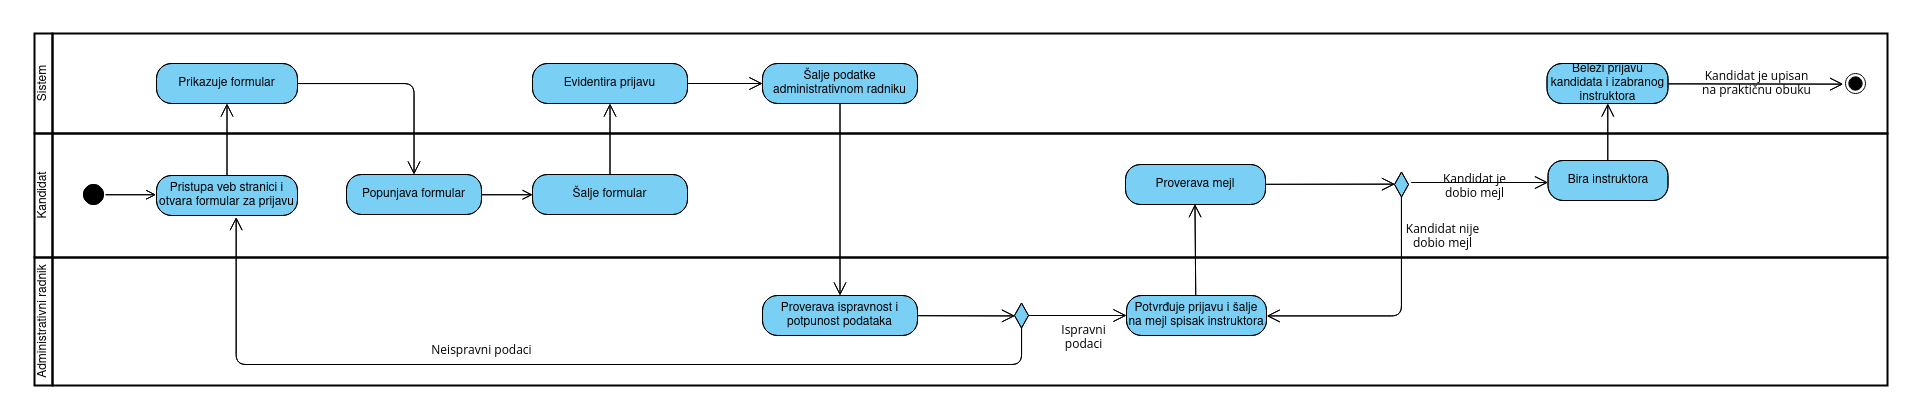
\includegraphics[width=140mm, height=70mm]{Diagrams/dijagram_aktivnosti_prijava_za_prakticnu_obuku.png}
  \end{center}
  \caption {Dijagram aktivnosti - Prijava za praktičnu obuku}
  \label{activity_prijava_za_prakticnu_obuku}

\end{figure}


\subsubsection{Pohađanje praktične obuke}

\vspace{3mm}

\begin{itemize}

\item \textbf{Kratak opis:} Kandidat sa instruktorom dogovara časove vožnje. Neophodno je da kandidat prisustvuje ukupno 40 časova i prisustvo se belezi u sistem.

\vspace{2mm}

\item \textbf{Učesnici} \newline
   - Kandidat \newline   
   - Instruktor 
   
\item \textbf{Preduslovi:} \newline
   - Kandidat je prijavljen za praktičnu obuku 

\item \textbf{Postuslovi:} \newline
    - Kandidat je završio praktičnu obuku.

\item \textbf{Osnovni tok:}  
   \begin{enumerate}
   \item Kandidat zakazuje čas u dogovoru sa instruktorom.
   \item Kandidat prisustvuje času u odgovarajućem terminu.
   \item Instruktor unosi podatke o održanom času.
   \item Kandidat potvrđuje prisustvo na času.
   \item Sistem čuva unete podatke. \newline
\textbf{Ovi koraci se ponavljaju za svih 40 časova.}
   \item Sistem šalje mejl kandidatu sa potvrdom o žavršenoj praktičnoj obuci.
   \item Kandidat otvara mejl i proverava da li je dobio potvrdu. 
   \item Sistem belezi da je kandidat zavrsio prakticnu obuku.
   \end{enumerate}

\item \textbf{Alternativni tok:}  
   \begin{itemize}
   \item A1. \textbf{Kandidat otkazuje čas:}
  Kandidat obaveštava instruktora da ne može da prisustvuje času i zakazuje novi termin časa, proces se nastavlja u koraku 1 osnovnog toka.
  \item A2. \textbf{Kandidat nije dobio potvrdu o završetku obuke:}
  Sistem nije poslao potvrdu kandidatu. Kandidat obaveštava administrativnog radnika da nije dobio mejl. Proces se nastavlja u koraku 6 osnovnog toka.
   \end{itemize}

\end{itemize}


\subsubsection{Prijava za praktični ispit}

\vspace{3mm}

\begin{itemize}

\item \textbf{Kratak opis:} Da bi kandidat izašao na vozački ispit prvo podnesi prijavu za polaganje. Popunjava online formular gde bira željeni termin, koji se  šalje administrativnom radniku. Nakon potvrde termina administrativni radnik šalje mejl sa terminom ispita i osnovnim info.

\vspace{2mm}

\item \textbf{Učesnici} \newline
   - Kandidat - korisnik sistema koji želi da se prijavi za praktični ispit.\newline   
   - Administrativni radnik - korisnik sistema koji proverava podatke, potvrđuje prijavu i šalje dodatne informacije kandidatu. 
   
\item \textbf{Preduslovi:} \newline
   - Sistem je u funkciji. \newline
   - Kandidat je položio prvu pomoć. \newline
   - Kandidat je dobio potvrdu o završenoj praktičnoj obuci. \newline
   - Kandidat je izvršio sve uplate

\item \textbf{Postuslovi:} \newline
    - Kandidat je prijavljen za izlazak na vozački ispit.

\item \textbf{Osnovni tok:}  
   \begin{enumerate}
   \item Kandidat otvara online formular za prijavu za izlazak na ispit.
   \item Sistem prikazuje formular.
   \item Kandidat bira termin za ispit.
   \item Kandidat se prijavljuje klikom na dugme "Pošalji".
   \item Sistem beleži prijavu za praktični ispit.
   \item Sistem šalje podatke administrativnom radniku.
   \item Administrativni radnik proverava da li kandidat ispunjava uslove za izlazak.
   \item Administrativni radnik šalje mejl kandidatu gde potvrđuje prijavu i dostavlja dodatne informacije.
   \item Kandidat otvara mejl i proverava da li je dobio potvrdu za izlazak na ispit. 
   \item Sistem beleži podatke o prijavi. 
   \end{enumerate}

\item \textbf{Alternativni tok:}  
   \begin{itemize}
   \item A1. \textbf{Nevalidni podaci:}
  Ukoliko u koraku 7 kandidat ne ispunjava uslove za prijavu na ispit, proces se prekida dok kandidat ne ispuni sve uslove za izlazak na ispit.
  \item A2. \textbf{Kandidat nije dobio potvrdu za izlazk na ispit:}
  Ukoliko u koraku 9 kandidat nije dobio mejl, obaveštava administrativnog radnika i proces se nastavlja u koraku 8 osnovnog toka.
   \end{itemize}

\end{itemize}  

\begin{figure}[H]
  \begin{center}
      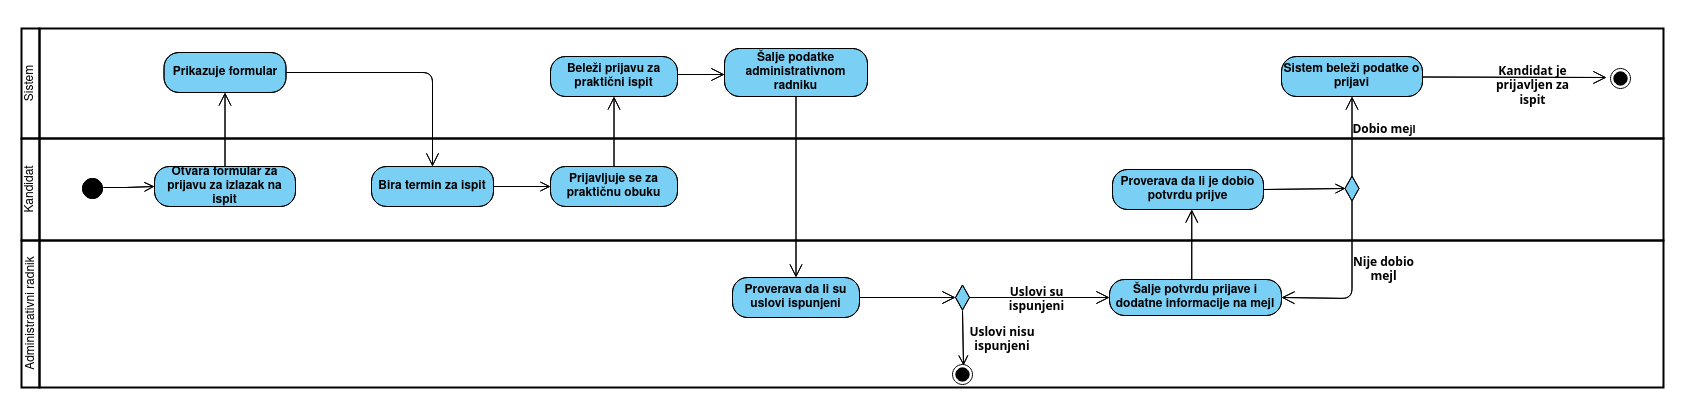
\includegraphics[width=140mm, height=70mm]{Diagrams/dijagram_aktivnosti_prijava_za_praktican_ispit.png}
  \end{center}
  \caption {Dijagram aktivnosti - Prijava za praktični ispit}
  \label{activity_prijava_za_prakticni_ispit}

\end{figure}


\subsubsection{Polaganje praktičnog ispita}

\vspace{3mm}

\begin{itemize}

\item \textbf{Kratak opis:} Kandidat polaže vozački ispit i nakon uspešnog polaganja popunjava anketu o auto školi i dobija potvrdu o položenom vozačkom ispitu.

\vspace{2mm}

\item \textbf{Učesnici} \newline
   - Kandidat \newline   
   - Instruktor \newline
   - Administrativni radnik 
   
\item \textbf{Preduslovi:} \newline
   - Kandidat se prijavio za praktični ispit.

\item \textbf{Postuslovi:} \newline
    - Kandidat je završio sa obukom.

\item \textbf{Osnovni tok:}  
   \begin{enumerate}
   \item Kandidat izlazi na završni ispit.
   \item Sistem prikazuje instruktoru putanju vožnje za tog kandidata.
   \item Instruktor saopštava putanju kandidatu.
   \item Kandidat vozi po datoj putanji.
   \item Kandidat uspešno završava vozački ispit.
   \item Instruktor saopštava broj poena.
   \item Instruktor potvrđuje položen ispit u sistemu.
   \item Kandidat popunjava anketu.
   \item Administrativni radnik šalje potvrdu o položenom vozakom ispitu.
   \item Kandidat ulazi na mejl i proverava potvrdu o položenom vozačkom ispitu.
   \item Sistem ažurira podatke o kandidatu.     

   \end{enumerate}

\item \textbf{Alternativni tok:}  
   \begin{itemize}
   \item A1. \textbf{Kandidat nije položio praktični ispit:}
  Kandidat nije ispunio sve zahteve i nije polozio prakticni ispit. Proces se prekida dok se kandidat opet ne prijavi za polaganje prakticnog ispita. 
  \item A2. \textbf{Kandidat nije dobio potvrdu o položenom ispitu:}
  Administrativni radnik nije poslao potvrdu kandidatu. Kandidat obaveštava administrativnog radnika da nije dobio mejl. Proces se nastavlja u koraku 9 osnovnog toka.
   \end{itemize}

\end{itemize}  


Na slici \ref{fig:bpmnP_podnosenje_zahteva} je prikazan BPMN dijagram procesa praktične nastave, 
na slici \ref{fig:bpmnS_podnosenje_zahteva} je prikazan BPMN dijagram saradnje praktične nastave, 
koji predstavljaju sled događaja u sistemu za 4 slučaja upotrebe:
\begin{itemize}
    \item Prijava za praktičnu obuku
    \item Pohađanje praktične obuke
    \item Prijava za praktični ispit
    \item Polaganje praktičnog ispita
\end{itemize}

\begin{figure}[H]
    \begin{center}
        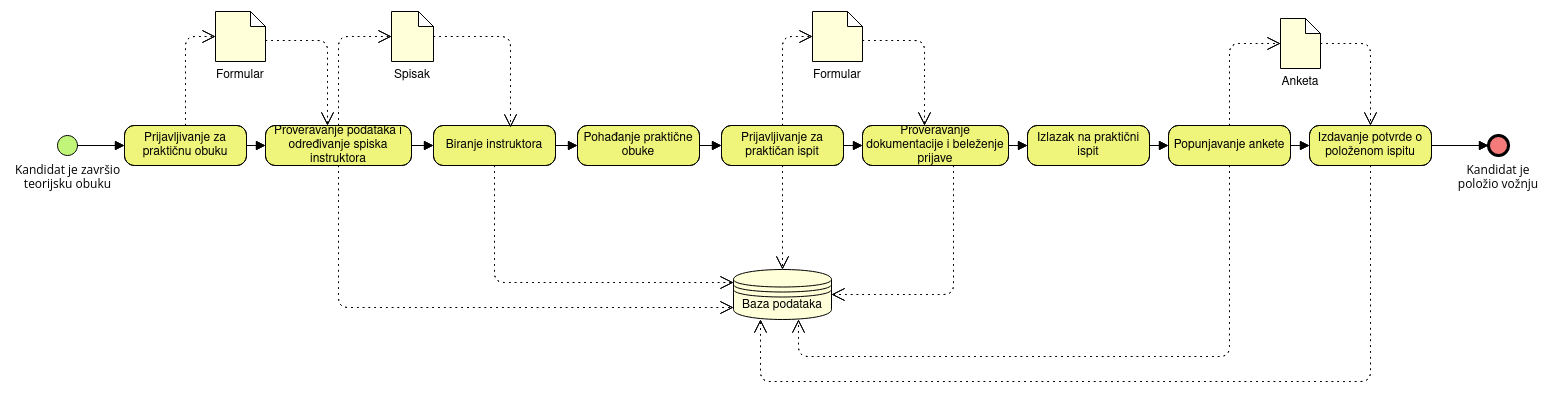
\includegraphics[width=120mm, height=60mm]{Diagrams/bpmnP_prakticna_nastava.png}
    \end{center}
    \caption {BPMN dijagram procesa praktične nastave}
    \label{fig:bpmnP_podnosenje_zahteva}

\end{figure}

\begin{figure}[H]
    \begin{center}
        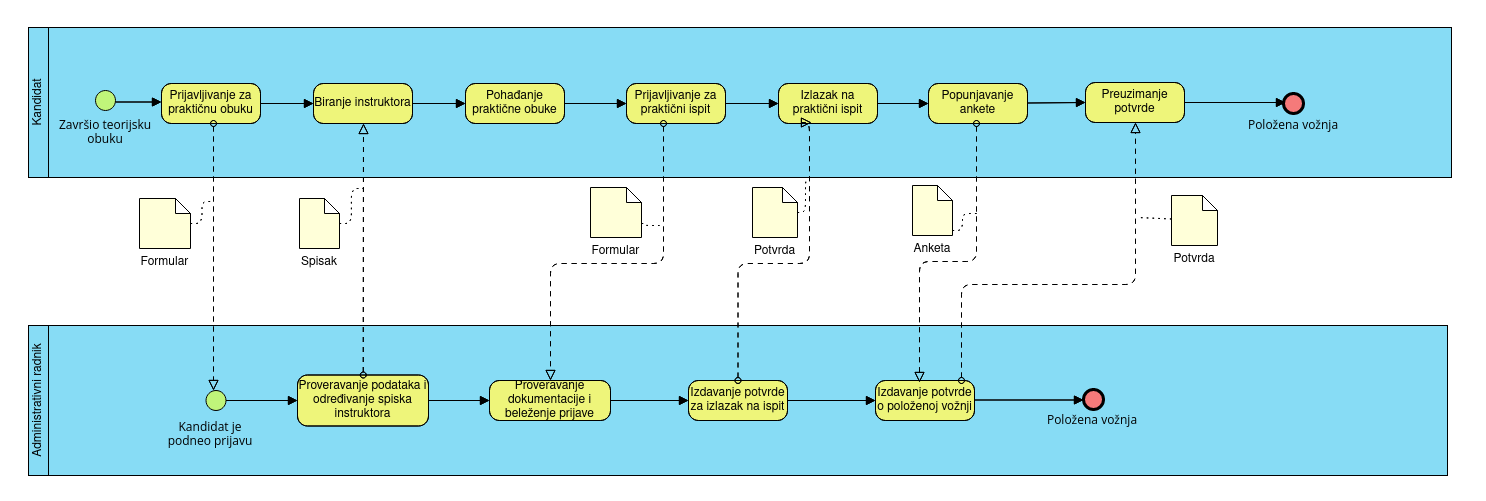
\includegraphics[width=120mm, height=60mm]{Diagrams/bpmnS_prakticna_nastava.png}
    \end{center}
    \caption {BPMN dijagram saradnje praktične nastave}
    \label{fig:bpmnS_podnosenje_zahteva}

\end{figure}

Kroz rad sistema kandidat prolazi kroz više različitih stanja. Na slici  \label{fig:stanja_kandidat} je prikazan dijagram stanja kanidata, 
koji obuhvata stanja kroz koja kandidat prolazi u celom procesu obuke (Podnošenje zahteva za prijavu, Teorijska obuka i Praktična obuka).

\begin{figure}[H]
    \begin{center}
        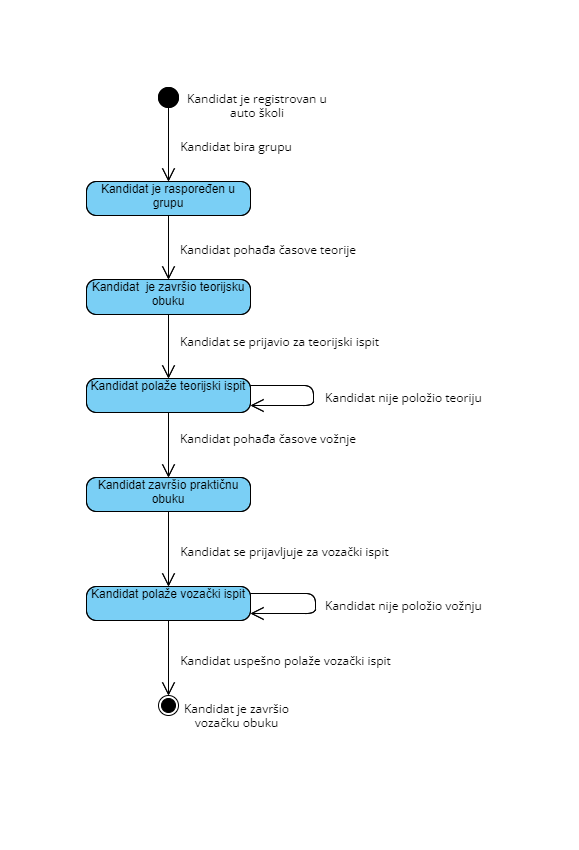
\includegraphics[height=100mm]{Diagrams/dijagram_stanja_kandidata.png}
    \end{center}
    \caption {Dijagram stanja kandidata}
    \label{fig:stanja_kandidat}

\end{figure}




\subsection {Vođenje evidencije}
Ovde ćemo predstaviti 3 slučaja upotrebe koje obavlja najvećim delom  nadležni za zaposlene i vrši vođenje različitih evidencija.
Pre svega predstavićemo administrativni deo auto škole, vođenje evidencije o invenatru škole i ostalim pokretnostima i nepokretnostima.
Nakon toga vođenje evidencija o zaposlenim kadrovima i njihovom rasporedu rada. Za kraj tu su i evidencije o polaganju ispita, odnosno formiranje 
odgovarajućih zapisnika o tim proverama.

\begin{figure}[H]
    \begin{center}
        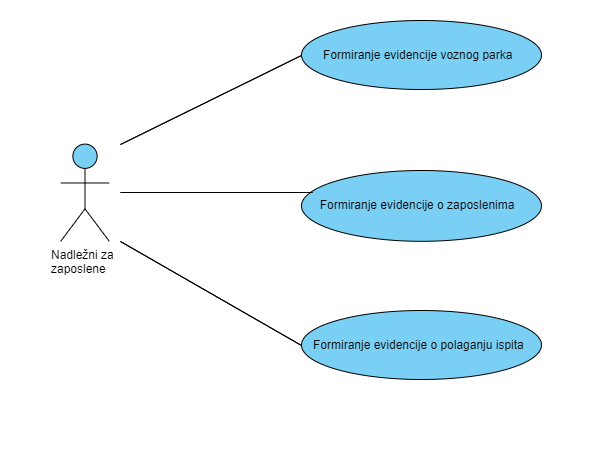
\includegraphics[width=120mm, height=60mm]{Diagrams/evidencija.png}
    \end{center}
    \caption {Praktična obuka}
    \label{usecase_praktična obuka}

\end{figure}

\subsubsection{Formiranje evidencija voznog parka}
\label{subsubsec:vozni park}
\begin{itemize}
  \item \textbf{Kratak opis}: Nadležni za zaposlene ima mogućnost da vodi evidenciju svih kola i instruktora, i da vrši promene u inventaru i rasporedu.
  \item \textbf{Učesnici}:
    \begin{itemize}
    \item Nadležni za zaposlene - korisnik sistema koji vrši raspored inventara i evidenciju.
    \end{itemize}
  \item \textbf{Preduslovi}:
    \begin{itemize}
    \item  Nadležni za zaposlene je uspešno ulogovan na sistem auto škole.
    \item  Sistem je u funkciji.
    \item  Nadležni za zaposlene ima pristup internetu.
    \end{itemize}
  \item \textbf{Postuslovi}:
      \begin{itemize}
      \item  Nadležni za zaposlene je ažurirao vozni park i dodelio vozilima instruktore.
      \end{itemize}
  \item \textbf{Osnovni tok}:
      \begin{enumerate}
        \item Nadležni za zaposlene otvara stranicu za uvid  u stanje voznog parka.
        \item Sistem prikazuje trenutni vozni park i informacije koji instruktor upravlja vozilom.
        \item Nadležni pritiska dugme "Izmeni"  na stranici.
        \item Sistem omogućava organizatoru da izmeni podatke u tabeli.
        \item Nadležni za zaposlene unosi izmene.
        \item Nadležni za zaposlene potvrđuje izmene.
        \item Sistem evidentira izmene.
        \item Sistem šalje mejl o izmenama instruktorima ako je došlo do novog rasporeda.
      \end{enumerate}

  \item \textbf{Alternativni tokovi}:
      \begin{itemize}
        \item A1. \textbf{Neuspela validacija.}
        Ukoliko u koraku 5 nadležni u formu o izmenama unese nevalidne podatke polja formulara koja su neispravna će biti crvena.
        Nakon što nadležni ažurira podatke nastavlja se čuvanje izmena. Proces se nastavlja u koraku 6.
      \end{itemize}
      
  \item \textbf{Specijalni zahtevi}:
      \begin{itemize}
        \item Podaci koji se čuvaju za vozila su id auta, marka, reg broj, insturktor, kilometraža. 
      \end{itemize}
\end{itemize}

\begin{figure}[H]
  \begin{center}
      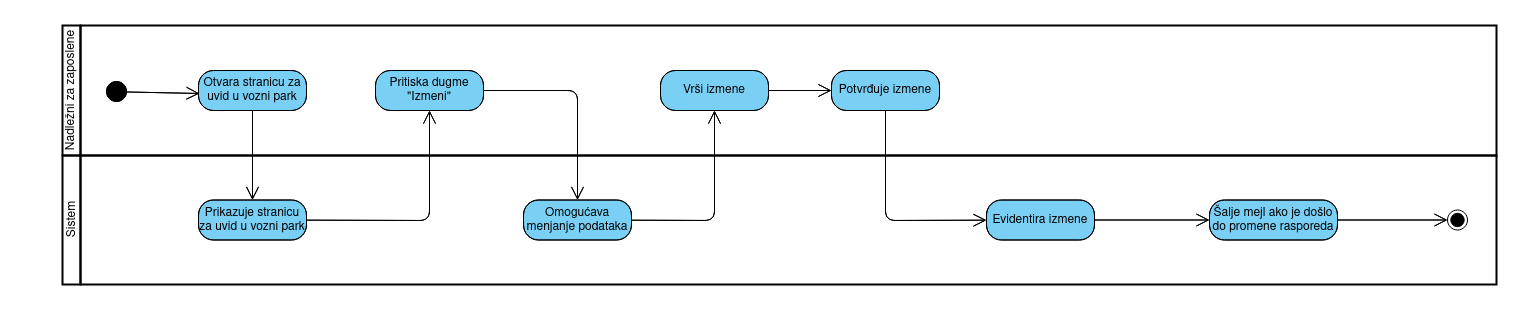
\includegraphics[width=170mm, height=70mm]{Diagrams/evidencija_vozila.png}
  \end{center}
  \caption {Dijagram aktivnosti - Formiranje evidencija voznog parka}
  \label{activity_evidencija_vozila}

\end{figure}

\subsubsection{Formiranje evidencije o zaposlenima}
\label{subsubsec:vozni park}
\begin{itemize}
  \item \textbf{Kratak opis}: Nadležni za zaposlene ima mogućnost da vodi evidenciju kadrova zaposlenih u auto školi 
  (instruktora, predavača, računovođa, administrativnih radnika). Vodi računa o rasporedu rada, radnom vremenu i slobodnim danima zaposlenih.

  \item \textbf{Učesnici}:
    \begin{itemize}
    \item Nadležni za zaposlene.
    \end{itemize}
  \item \textbf{Preduslovi}:
    \begin{itemize}
    \item  Nadležni za zaposlene je uspešno ulogovan na sistem auto škole.
    \item  Sistem je dostupan.
    \item  Nadležni za zaposlene ima pristup internetu.
    \end{itemize}
  \item \textbf{Postuslovi}:
      \begin{itemize}
      \item  Nadležni za zaposlene je ažurirao evidenciju o zaposlenim kadrovima u auto školi.
      \item  Nadležni za zaposlene je ažurirao evidenciju o rasporedu rada zaposlenih.
      \end{itemize}
  \item \textbf{Osnovni tok}:
      \begin{enumerate}
        \item Nadležni za zaposlene otvara stranicu za uvid u spisak zaposlenih radnika.
        \item Sistem prikazuje trenutno zaposlene kao i njihov raspored rada za tekuću nedelju ili dan.
        \item Nadležni pritiska dugme "Izmeni" na stranici.
        \item Sistem omogućava organizatoru da izmeni podatke u tabeli ili doda nove.
        \item Nadležni dodaje novog zaposlenog na spisak ili menja radno vreme nekom zaposlenom po potrebi.
        \item Nadležni potvrđuje izmene.
        \item Sistem evidentira izmene.
        \item Sistem šalje mejl o izmenama zaposlenima ako je došlo do novog rasporeda rada za narednu nedelju ili dan.
      \end{enumerate}

  \item \textbf{Alternativni tokovi}:
      \begin{itemize}
        \item A1. \textbf{Neuspela validacija.}
        Ukoliko u koraku 5 nadležni u formu o izmenama unese nevalidne podatke polja formulara koja su neispravna će biti crvena.
        Nakon što nadležni ažurira podatke nastavlja se čuvanje izmena. Proces se nastavlja u koraku 6.
      \end{itemize}

      
  \item \textbf{Dodatne informacije}:
      \begin{itemize}
        \item Podaci o zaposlenom : ime, prezime, jmbg, broj telefona, raspored rada.
      \end{itemize}
\end{itemize}

\begin{figure}[H]
  \begin{center}
      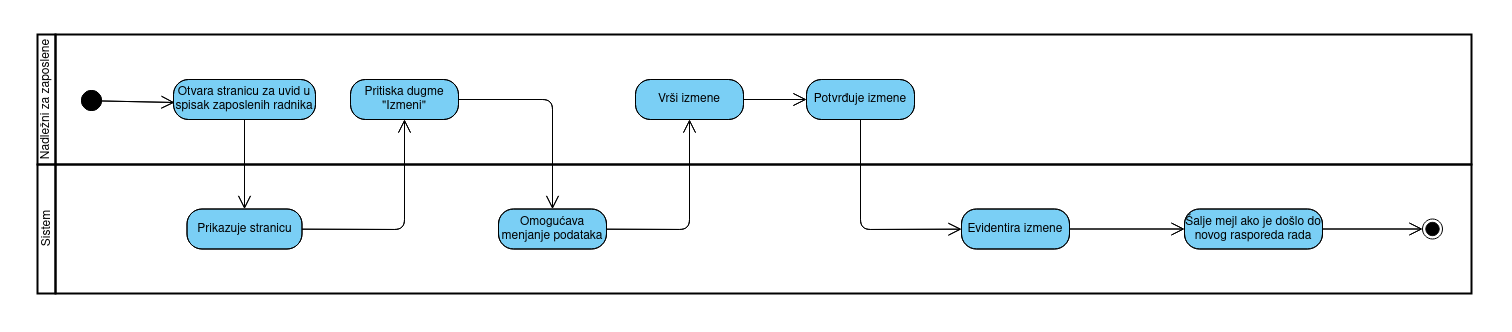
\includegraphics[width=140mm, height=70mm]{Diagrams/evidencija_zaposlenih.png}
  \end{center}
  \caption {Dijagram aktivnosti - Formiranje evidencije o zaposlenima}
  \label{activity_evidencija_zaposlenih}

\end{figure}

\subsubsection{Formiranje evidencije o polaganju ispita}
\label{subsubsec:vozni park}
\begin{itemize}
  \item \textbf{Kratak opis}: Nadležni za zaposlene ima mogućnost da vodi evidenciju o polaganju praktičnog ispita. Vodi računa o vremenu kad se održava ispit, instrukoru koji je zadužen za polaganje, kandidatu koji polaže ispit i o anketi koju kandidat popunjava na kraju ispita.

  \item \textbf{Učesnici}:
    \begin{itemize}
    \item Nadležni za zaposlene.
    \end{itemize}
  \item \textbf{Preduslovi}:
    \begin{itemize}
    \item  Nadležni za zaposlene je uspešno ulogovan na sistem auto škole.
    \item  Sistem je dostupan.
    \item  Nadležni za zaposlene ima pristup internetu.
    \end{itemize}
  \item \textbf{Postuslovi}:
      \begin{itemize}
      \item  Nadležni za zaposlene je ažurirao evidenciju o ispitu.
      \item  Nadležni za zaposlene je ažurirao evidenciju o instruktorima, na osnovu anketa.
      \end{itemize}
  \item \textbf{Osnovni tok}:
      \begin{enumerate}
        \item Nadležni za zaposlene otvara stranicu za uvid u spisak prijavljenih kandidata.
        \item Nadležni za zaposlene beleži u sistem prisustvo kandidata.
        \item Nadležni za zaposlene beleži vreme početka ispita i dodeljenog instruktora u sistem.
        \item Sistem pamti podatke.
        \item Nadležni unosi u sistem rezultate ispita.
        \item Nadležni za zaposlene prosleđuje anketu kandidatu.
        \item Nadležni za zaposlene unosi podatke iz ankete i ažurira evidencije o instruktorima.
        \item Sistem potvrđuje izmene.
      \end{enumerate}

  \item \textbf{Alternativni tokovi}:
      \begin{itemize}
        \item A1. \textbf{Kandidat nije položio.}
        Ukoliko je u koraku 5 nadležni uneo u sistem da je kandidat pao vožnju, proces se prekida.
      \end{itemize}
      
  \item \textbf{Dodatne informacije}:
      \begin{itemize}
        \item Kandidat popunjava anketu o svom iskustu u auto školi i svom iskustu sa izabranim instruktoram.
      \end{itemize}
\end{itemize}



\subsection {Vođenje finansija}
Ovde ćemo predstaviti slučajeve upotrebe koje obavlja najvećim delom računovođa u auto školi.
To podrazumeva vođenje evidencije o isplati plata zaposlenima, uplatama kandidata, kao i održavanje tekućeg cenovnika usluga u auto školi.

\subsubsection{Pregled plata zaposlenih}
\label{subsubsec:vozni park}
\begin{itemize}
  \item \textbf{Kratak opis}: Računovođa može da zatraži pregled plata zaposlenih u određenom vremenskom trenutku. Kada dobije željeni izveštaj, 
  može ga sačuvati na sistemu, izmeniti ili odštampati.

  \item 
  \item \textbf{Učesnici}:
    \begin{itemize}
    \item Računovođa.
    \end{itemize}
  \item \textbf{Preduslovi}:
    \begin{itemize}
    \item  Računovođa je uspešno ulogovan na sistem auto škole.
    \item  Sistem je dostupan.
    \item  Računovođa ima pristup internetu.
    \end{itemize}
  \item \textbf{Postuslovi}:
      \begin{itemize}
      \item  Računovođa je dobio izveštaj o zahtevanim platama za zaposlene.
      \item  Računovođa je uspešno izvršio željene izmene plata.
      \end{itemize}
  \item \textbf{Osnovni tok}:
      \begin{enumerate}
        \item Računovođa otvara stranicu za uvid u spisak zaposlenih radnika i njihovih plata u željenom periodu.
        \item Sistem prikazuje trenutno zaposlene kao i njihove plate.
        \item Računovođa bira dugme "Izmeni" da promeni platu ili  "Odštampaj" za dobijanje izveštaja.
        \item Sistem omogućava računovođi da izmeni podatke u tabeli  ili  izvrši štampanje.
        \item Računovođa potvrđuje izmene ili vrši štampanje.
        \item Sistem evidentira izmene.
      \end{enumerate}

  \item \textbf{Alternativni tokovi}:
      \begin{itemize}
        \item A1. \textbf{Ne mogu se dobiti traženi podaci.}
        Ako sistem u koraku 2 ne može iz nekog razloga da prikaže tražene podatke, računovođa se obaveštava da je došlo do problema.
        Proces se nastavlja od koraka 1 osnovnog toka.
        \item A1. \textbf{Neuspela izmena ili štampanje.}
        Ako u koraku 5 štampač nije dostupan ili su uneti podaci nevalidni, računovođa se obaveštava o problemu. Proces se nastavlja unošenjem
        validnih podataka u slučaju izmene i nastavlja se od koraka 4. U slučaju nedostupnosti štampača proces se završava.
      \end{itemize}

      
  \item \textbf{Dodatne informacije}:
      \begin{itemize}
        \item Podaci o zaposlenom : ime, prezime, jmbg, broj telefona, plata.
      \end{itemize}
\end{itemize}

\subsubsection{Pregled cena usluga}
\label{subsubsec:vozni park}
\begin{itemize}
  \item \textbf{Kratak opis}: Računovođa vodi računa o cenana usluga i mogućim popustima

  \item \textbf{Učesnici}:
    \begin{itemize}
    \item Računovođa.
    \item Kandidat.
    \end{itemize}
  \item \textbf{Preduslovi}:
    \begin{itemize}
    \item  Kandidat želi da se upiše u auto školu.
    \end{itemize}
  \item \textbf{Postuslovi}:
      \begin{itemize}
      \item  Kandidatu je određena cena obuke.
      \end{itemize}
  \item \textbf{Osnovni tok}:
      \begin{enumerate}
        \item Kandidat donosi osnovne podatke računovođi.
        \item Računovođa saopštava osnovnu cenu obuke.
        \item Računovođa određuje popust za datog kandidata.
        \item Računovođa saopštava cenu obuke sa popustom.
        \item Kandidat nastavlja sa upisom.
      \end{enumerate}

  \item \textbf{Alternativni tokovi}:
      \begin{itemize}
        \item A1. \textbf{Kandidat ne prihvata cenu obuke:}
        Kandidatu ne odgovara cena obuke. Proces se prekida.
      \end{itemize}

      
  \item \textbf{Dodatne informacije}:
      \begin{itemize}
        \item Računovođa oređuje popust na osnovu socijalno ekonomskog statusa i na osnovu pripadnosti društveno osetljivim grupama.
      \end{itemize}
\end{itemize}

\begin{figure}[H]
  \begin{center}
      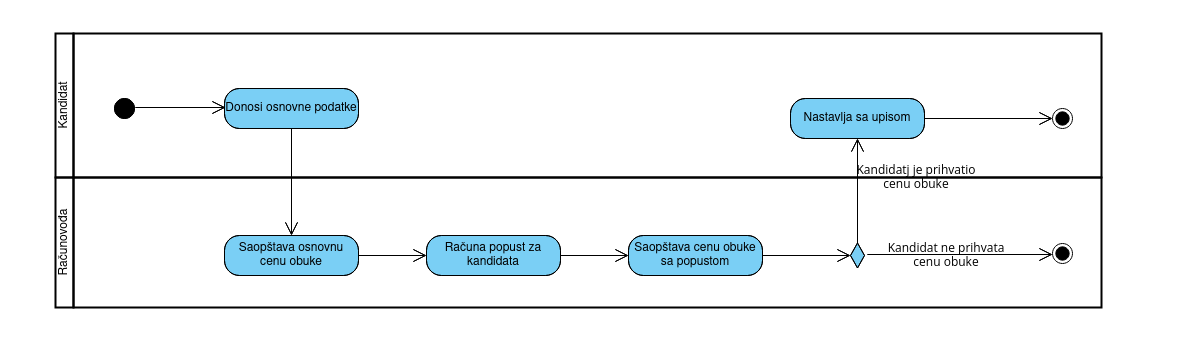
\includegraphics[width=140mm, height=70mm]{Diagrams/dijagram_aktivnosti_cena_obuke.png}
  \end{center}
  \caption {Dijagram aktivnosti - Pregled cena usluga}
  \label{activity_pregled_cena_usluga}

\end{figure}




\section {Opis baze podataka}
\label{sec:database}

Putem dijagrama klasa na slici \ref{fig:dijagram_klasa} je predstavljena baza.

U bazi su predstavljeni podaci podeljeni u 4 grupe podataka:
\begin{itemize}
    \item Podaci o osoblju i kandidatu
    \item Podaci o ispitu
    \item Podaci o nastavi
    \item Ostali podaci
\end{itemize}


\subsection{Podaci o osoblju i kandidatu}

\textbf{\large Osoba}
\vspace{0.3cm}

Klasa \textit{Osoba} predstavlja osnovne informacije o korisnicima našeg sistema. 
Iz ovog tipa entiteta primenom specijalizacije izvodimo 2 nova tipa entiteta: Osoblje i Kandidat.

Atributi:
\begin{itemize}
    \item id - jedinstveni identifikator korisnika (PK, automatski generisan)
    \item lozinka 
    \item ime
    \item prezime
    \item jmbg
    \item pol
    \item telefon
\end{itemize}

\textbf{\large Osoblje}
\vspace{0.3cm}

Klasa \textit{Osoblje} predstavlja zaposlene osobe u našem sistemu.
Iz ovog tipa entiteta primenom specijalizacije izvodimo 6 novih tipova entiteta: 
Predavač, Instruktor, Nadležni za zaposlene, Računovođa, Administrativni radnik i Administrator sistema.

Atributi:
\begin{itemize}
    \item brojRačuna
    \item visinaPlate
    \item datumZaposlenja
\end{itemize}

\textbf{\large Kandidat}
\vspace{0.3cm}

Klasa \textit{Kandidat} predstavlja jednog kandidata koji je upisan u auto školu.

Atributi:
\begin{itemize}
    \item datumRođenja
    \item datumUpisa
    \item idInstruktora - instruktor koji drži kandidatu časove vožnje (SK koji referiše na Instruktor)
    \item idGrupe - grupa u koju je kandidat raspoređen (SK koji referiše na Grupa)
\end{itemize}


\textbf{\large Instruktor}
\vspace{0.3cm}

Klasa \textit{Instruktor} predstavlja zaposlenog koji je zadužen da drži časove praktične nastave.

Atributi:
\begin{itemize}
    \item idVozila - vozilo koje je dodeljeno instruktoru (SK koji referiše na Vozilo)
    \item ocena - trenutna ocena za instruktora na osnovu rezultata ankete
\end{itemize}

\subsection{Podaci o nastavi}

\textbf{\large Nastava}
\vspace{0.3cm}

Klasa \textit{Nastava} predstavlja osnovne informacije o nastavi u auto školi. Iz ovog tipa entiteta primenom specijalizacije izvodimo 2 nova tipa entiteta: Praktična nastava i Teorijska nastava.

Atributi:
\begin{itemize}
    \item id - jedinstveni identifikator ispita (PK, automatski generisan)
    \item datumOdržavanja
    \item vremeOdržavanja
\end{itemize}

\textbf{\large Teorijska nastava}
\vspace{0.3cm}

Klasa \textit{Teorijska nastava} predstavlja osnovne informacije vezano za teorijsku nastavu.

Atributi:
\begin{itemize}
    \item idPredavača (SK koji referiše na Predavač)
    \item brojSale
    \item idGrupe (SK koji referiše na Grupa)
\end{itemize}

\textbf{\large Praktična nastava}
\vspace{0.3cm}

Klasa \textit{Praktična nastava} predstavlja osnovne informacije vezano za praktičnu nastavu.

Atributi:
\begin{itemize}
    \item idInstruktora (SK koji referiše na Instruktor)
    \item brojRute
    \item idKandidata (SK koji referiše na Kandidat)
    \item nocnaVoznja
    \item idVozila (SK koji referiše na Vozilo)
\end{itemize}


\subsection{Podaci o ispitu}

\textbf{\large Ispit}
\vspace{0.3cm}

Klasa \textit{Ispit} predstavlja osnovne informacije o ispitu. 
Iz ovog tipa entiteta primenom specijalizacije izvodimo 2 nova tipa entiteta: Praktični ispit i Teorijski ispit.
Klasa \textit{Teorijski ispit} predstavlja osnovne informacije vezano za polaganje teorijskog ispita.
Klasa \textit{Praktični ispi} predstavlja osnovne informacije vezano za polaganje praktičnog ispita.

Atributi:
\begin{itemize}
    \item id - jedinstveni identifikator ispita (PK, automatski generisan)
    \item datumPolaganja 
    \item vremePolaganja
    \item idKandidata - koji polaže praktični/teorijski ispit(SK koji referiše na Kandidat)
    \item statusPolaganja
    \item brojPoena 
\end{itemize}






\subsection{Ostali podaci}

\textbf{\large Vozilo}
\vspace{0.3cm}

Klasa \textit{Vozilo} predstavlja osnovne informacije o stanju vozila

Atributi:
\begin{itemize}
    \item id - jedinstveni identifikator ispita (PK, automatski generisan)
    \item registracioniBroj
    \item model
    \item datumRegistracije
    \item pređeniKm
\end{itemize}

\textbf{\large Anketa}
\vspace{0.3cm}

Klasa \textit{Anketa} predstavlja jednu anketu koju kandidat popunjava unoseći utiske o instruktoru.

Atributi:
\begin{itemize}
    \item id (PK, automatski generisan)
    \item idKandidata - kandidat koji popunjava anketu (SK koji referiše na Kandidat)
    \item ocena - ocena koju daje instruktoru
\end{itemize}

\textbf{\large Grupa}
\vspace{0.3cm}

Klasa \textit{Grupa} predstavlja osnovne informacije o jednoj polaznoj grupi kandidata koji pohađaju teorijsku nastavu.

Atributi:
\begin{itemize}
    \item id (PK, automatski generisan)
    \item brojKandidata 
    \item idPredavača - predavač koji je dodeljen grupi (SK koji referiše na Predavač)
\end{itemize}

Klasa \textit{Uplata} predstavlja podatke o jednoj uplati kandidata, u određenom iznosu, po cenovniku usluga auto škole.

Atributi:
\begin{itemize}
    \item id (PK, automatski generisan)
    \item idRačunovođe - računovođa koji evidentira uplatu (SK koji referiše na Računovođa)
    \item idKandidata - kandidat koji vrši uplatu u određenom iznosu (SK koji referiše na Kandidat)
    \item iznos
    
\end{itemize}




\begin{figure}[H]
    \begin{center}
        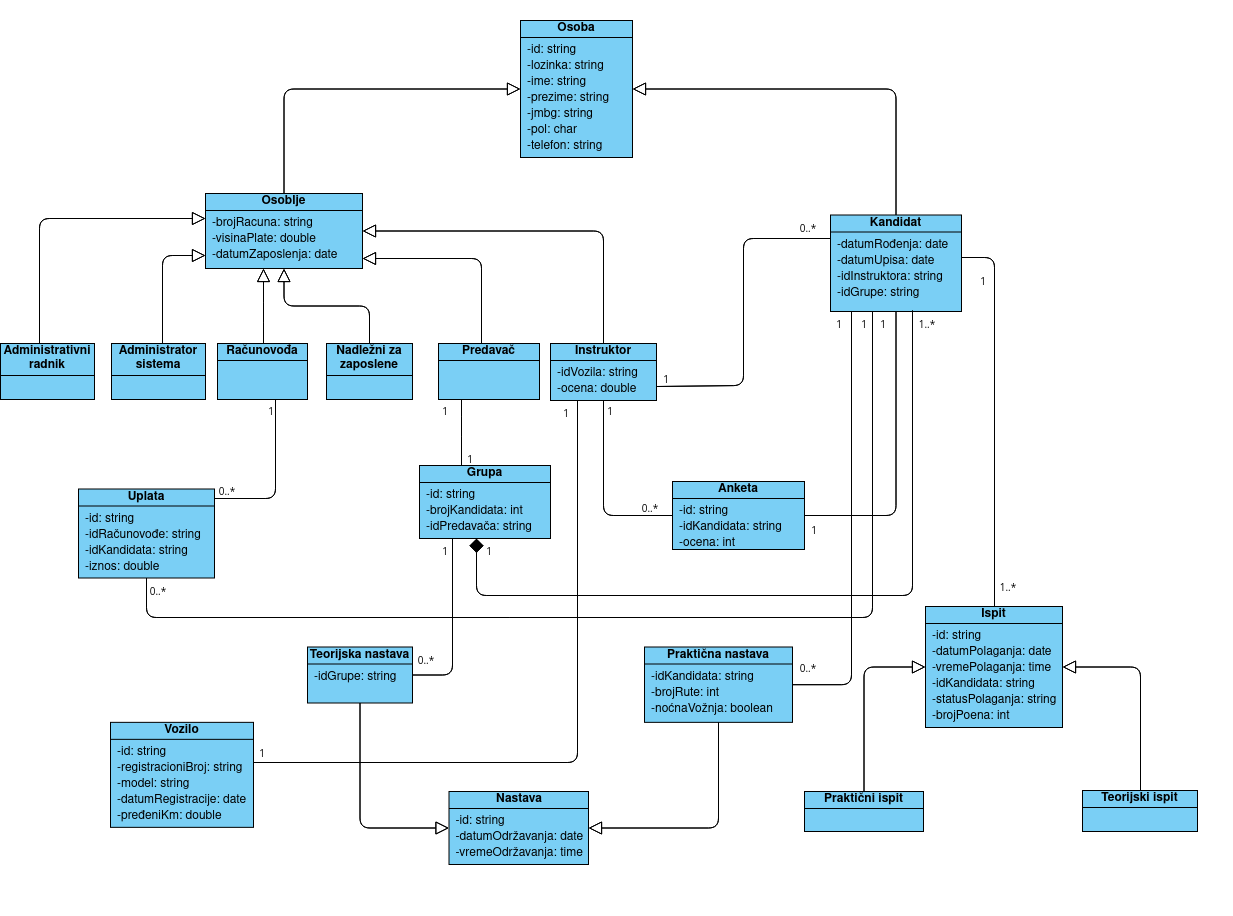
\includegraphics[width=\textwidth]{Diagrams/dijagram_klasa.png}
        \caption {Dijagram klasa baze podataka}
        \label{fig:dijagram_klasa}
    \end{center}
\end{figure}

\section{\bfseries Arhitektura sistema}

\subsection{Odabir arhitekture}
U ovom poglavlju predstavićemo arhitekturu našeg sistema. 
Izabraćemo najpogodniju moguću arhitekturu sa balansom koji odgovara potrebama našeg sistema.
Pri odabiru uzeti su u obzir osnovni zahtevi postavljeni pred arhitekturu : funkcionalni zahtevi - šta sistem treba da radi i zahtevi o kvalitetu.
Arhitektura je odabrana tako da ispuni što  je više moguće od sledećih zahteva:
\begin{itemize}
    \item Bezbednost sistema
    \item Lakoća korišćenja
    \item Brzina odziva
    \item Dostupnost
    \item Pouzdanost
\end{itemize}

Karakteristike arhitekture sistema:
\begin{enumerate}
    \item Tip aplikacije : Veb aplikacija
    \item Strategije isporučivanja: Jedan serverski i više klijentskih računara
    \item Tehnologije: Node.js, relaciona baza podataka

\end{enumerate}

\subsection{Tip i slojevi arhitekture}
Na osnovu prethodno navedene analize, odabrana je klijent-server arhitektura i aplikacija se sastoji iz 3 sloja:
\begin{enumerate}
\item Prezentacioni sloj
\item Logički sloj
\item Sloj podataka
\end{enumerate}

\subsubsection{Prezentacioni sloj}

Ovo je najviši sloj aplikacije i njegova uloga je prikazivanje korisniku vizuelnog sadržaja,
koristeći podatke koje dobija od nižeg sloja.
Zadužen je da korisniku obezbedi što lakšu i efikasniju upotrebu aplikacije.
Funkcionalnosti koje pruža razlikuju se u zavisnosti od uloge korisnika i pokrivaju najvažnije slučajeve upotrebe 
Čine ga komponente koje korisnik vidi i sa kojima interaguje kroz veb pregledač i to su:

\begin{itemize}
    \item Registracija
    \item Prijavljivanje
    \item Odabir termina za praktični i teorijski ispit
\end{itemize}


\subsubsection{Logički sloj}

Logički sloj je središnji sloj i on se sastoji od Klijentskog kontrolera i Serverskog kontrolera.
Primarni zadatak klijentskog kontrolera jeste pouzdana komunikacija sa serverskim slojem sistema. 
Još jedan njegov zadatak je prosleđivanje podataka prezentacionom sloju, kako bi on prikazao korisniku vizuelni sadržaj.
Njegove komponente su sledeće:

\begin{itemize}
    \item Autorizacija i autentifikacija
    \item Dohvatanje podataka sa servera
    \item Validacija korisničkih podataka
\end{itemize}


Zadatak serverskog kontrolera je sličan kao kod klijentskog, s tim što se ovde vrši dodatna autentifikacija 
i autorizacija. To je omogućeno jer ovoj komponenti nemaju pristup klijenti i time se postiže bezbednost.
Takođe, ovde se vrši komunikacija sa bazom podataka.
Njegove komponente su sledeće:

\begin{itemize}
    \item Autorizacija i autentifikacija
    \item Dohvatanje podataka
    \item Pregled i izmene podataka 
\end{itemize}

\subsubsection {Sloj podataka}

Baza podataka čuva sve podatke koji su neophodni za sistem i ona je kao komponenta deo ovog sloja.
Takođe, ovaj sloj sadrži i sve neophodne mehanizme za pristup bazi podataka.
Opis baze podataka se nalazi u sekciji \ref{sec:database}.


\begin{figure}[H]
  \begin{center}
      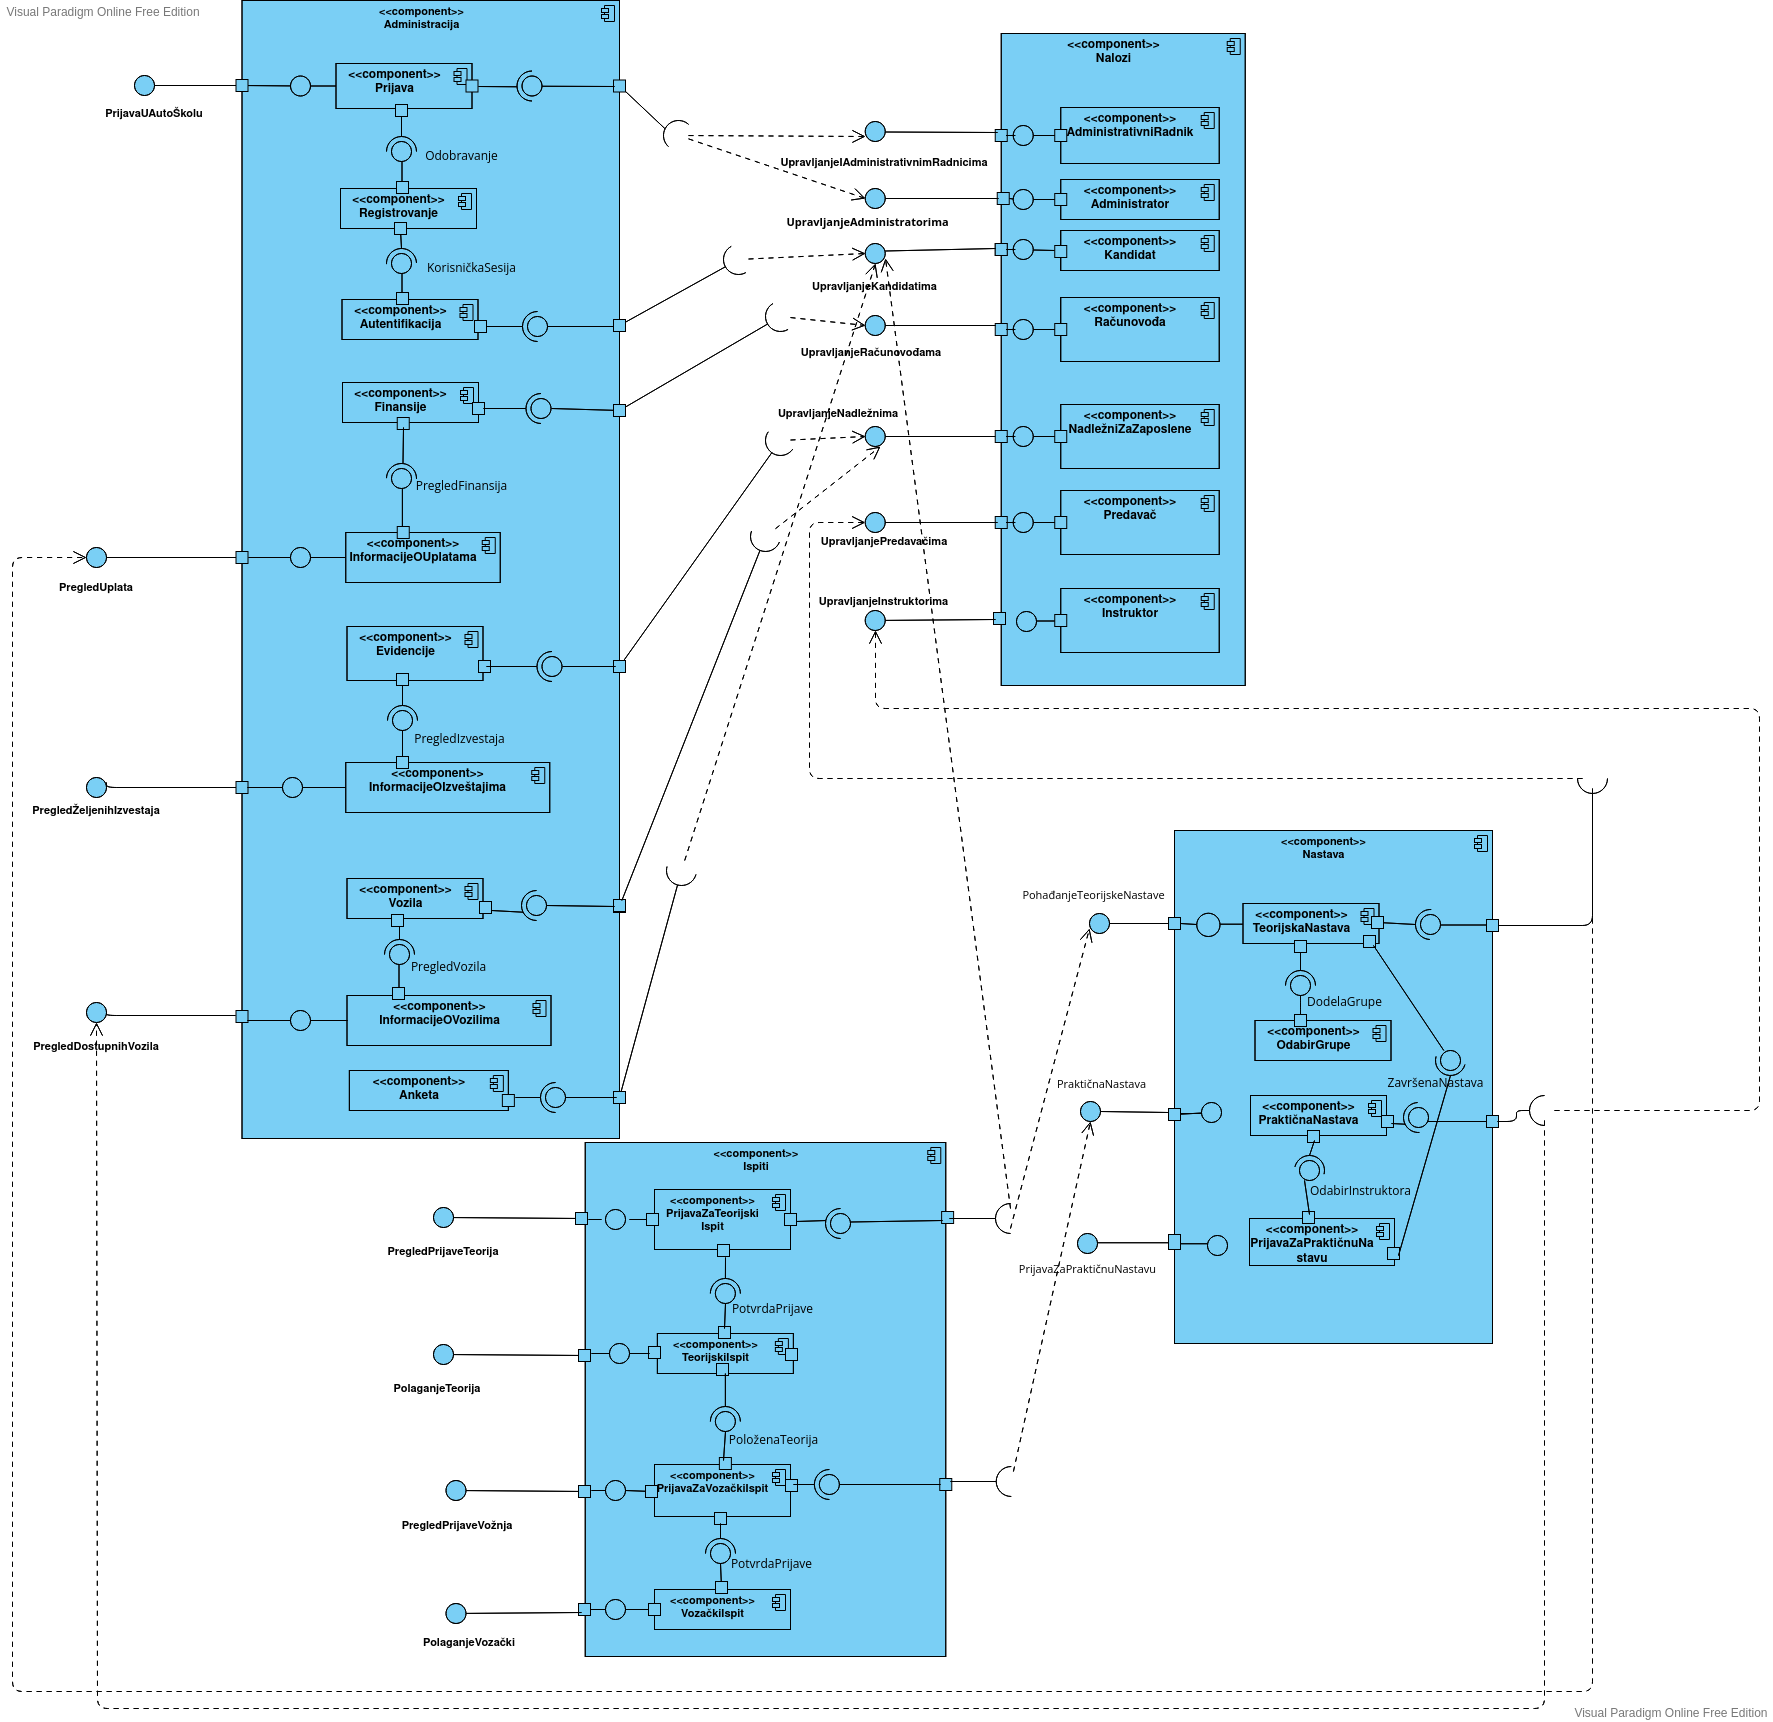
\includegraphics[width=\textwidth]{Diagrams/dijagram_komponenti.png}
  \end{center}
  \caption {Dijagram komponenti}
  \label{activity_dijagram_komponenti}

\end{figure}




\section{Zaključak}
\label{sec:zakljucak}


\addcontentsline{toc}{section}{Literatura}
\appendix
\bibliography{seminarski} 
\bibliographystyle{plain}





\end{document}
